\documentclass[12pt, letterpaper]{article}

\usepackage[margin=1in]{geometry}
\usepackage{graphicx}
\usepackage{float}
\usepackage{parskip}
\usepackage[T1]{fontenc}
\usepackage{lmodern}
\usepackage{hyperref}

\graphicspath{{images/}}

\title{\textbf{Servo Control Software}}
\author{ESC204, Engineering Science Praxis III \\ University of Toronto}
\date{March 2026}

\begin{document}
\maketitle

\section*{Overview}

The servo deployment mechanism is controlled using MicroPython running on the Raspberry Pi
Pico. The control code, shown in Figure~\ref{fig:code}, is adapted from the \texttt{servo.py}
reference provided in Lab 4 [1] and targets the electrical circuit design described in that
same lab. It drives each servo by writing a PWM duty cycle to the assigned GPIO pin, mapping
a target angle to the corresponding 1\,ms to 2\,ms pulse width at 50\,Hz.

For the deployment system, this code is applied to two servo instances on separate GPIO pins:
one for the MG996R linear actuation servo and one for the DF9GMS latch key servo. No changes
to the underlying PWM logic are required since both servos use the same standard control
protocol; only the pin assignments and target angles differ between the two.

\begin{figure}[H]
    \centering
    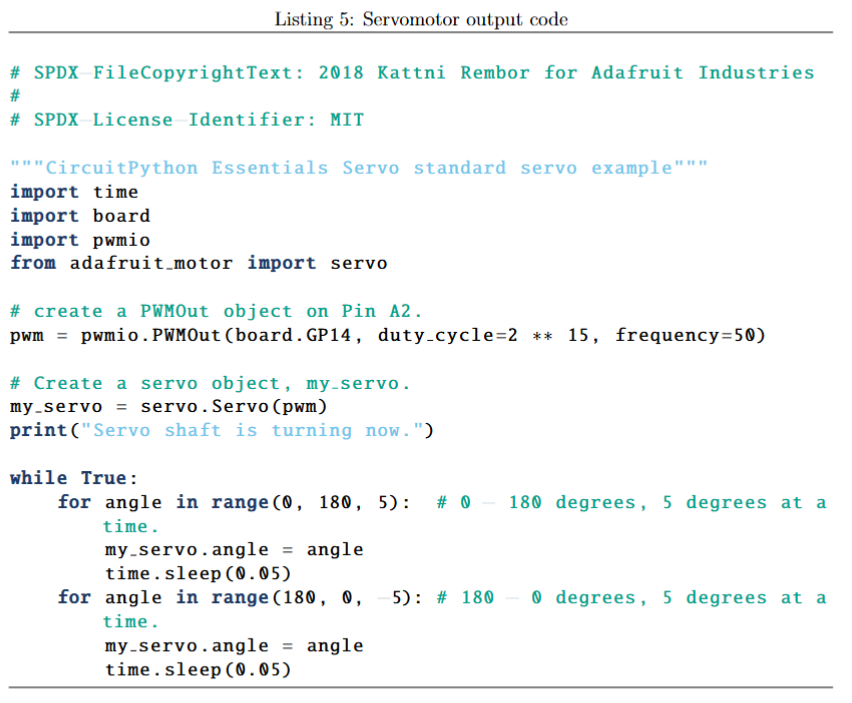
\includegraphics[width=0.82\textwidth]{code.png}
    \caption{Servo control code adapted from the Lab 4 \texttt{servo.py} reference [1].}
    \label{fig:code}
\end{figure}

\begin{thebibliography}{9}
\bibitem{lab4}
University of Toronto Engineering Science,
\textit{ESC204S Winter 2026 Lab 4 Instructions},
Version 1.0, January 29, 2026.
\end{thebibliography}

\end{document}
